Bevor in den folgenden Kapiteln Einblicke in die interne Struktur des Plugins (s. Kapitel \ref{cha:interne-struktur}) und die Verwendung des Plugins (s. Kapitel \ref{cha:verwendung}) gegeben werden, fasst dieses Kapitel die dem Projekt zu Grunde liegenden Anforderungen zusammen (s. Kapitel \ref{sec:anforderungen}) und stellt die zwei Schnittstellen vor, die am elementarsten für die Umsetzung des Projektes waren (s. Kapitel \ref{sec:schnittstellen}).

\section{Anforderungen}
\label{sec:anforderungen}

Grundlage für das \eigenname{\textbf{Q}uestion \textbf{P}lugin for \textbf{I}lias - \textbf{SQL} \textbf{(QPI-SQL)}} Projekt war die Idee, ein Plugin für \eigenname{ILIAS} zu entwickeln, dass es Studenten ermöglicht \eigenname{SQL} direkt in einem eigens entwickelten Fragentyp auszuführen und dabei auch eine automatische Korrektur der Antwort zu ermöglichen. Einige weitere Anforderungen kristallisierten sich in der Anfangsphase des Projektes heraus:

\begin{description}
    \item[Unabhängigkeit von Plugins] 
    Das zu entwickelnde Plugin für \eigenname{ILIAS} soll keine anderen Plugins in \eigenname{ILIAS} voraussetzen. So wird verhindert, dass Adminstratoren mehr als nötig in ihre \eigenname{ILIAS} Umgebung installieren müssen.
    
    \item[Keine serverseitige Ausführung von \eigenname{SQL}] 
    Wenn Studenten \eigenname{SQL} Code schreiben und diesen auch ausführen können sollen, so darf diese Ausführung nicht serverseitig erfolgen. Die Integrität des Servers kann so besser geschützt werden.
    
    \item[Verwendung von standardisierten Webtechnologien] 
    Um eine Nutzung des Plugins unabhängig von Gerät und Browser zu ermöglichen, soll das Plugin auf Seiten des Clients nur Technologien nutzen, die zum allgemeinen Standard eines aktuellen Browsers gehören.
    
    \item[Anpassbarkeit der automatischen Korrektur über Metriken] 
    Die automatische Korrektur von \eigenname{SQL} ist eines der Kernelemente des zu entwickelnden Plugins. Dem Ersteller von Fragen soll dabei die Möglichkeit gegeben werden die Bewertungskriterien zu steuern. Dazu soll die Bewertung auf Basis von unterschiedlichen Metriken erfolgen, die vom Ersteller gewichtet werden können. Als Basis für die Metriken soll  Wahl et al. \cite{WahlAndreas} dienen.
\end{description}


\section{Abhängigkeiten}
\label{sec:schnittstellen}

Eine der zwei grundlegenden Abhängigkeiten des \eigenname{QPI-SQL} Projektes ist die Plugin-API von \eigenname{ILIAS}. Während sich diese Schnittstelle direkt aus den Anforderungen ableiten lässt, stellte die Anforderung, dass \eigenname{SQL} zwar von Studenten ausgeführt werden soll, aber dabei weder serverseitige Datenbanken zur Verfügung stehen, noch clientseitige Programme oder Browserplugins, die Grundlage für die Verwendung der zweiten Abhängigkeit. Als anerkannter Webstandard bietet Javascript die Möglichkeit dynamische Berechnungen direkt im Browser auszuführen. \eigenname{SQL.js} ist eine zu Javascript kompilierte Variante des Datenbanksystems \eigenname{SQLite} (s. \cite{SQLjs}) und bietet somit im Rahmen der Anforderungen die Möglichkeit \eigenname{SQL} auszuführen.

Dieses Kapitel gibt einen kurzen Überblick über die Verwendung der \eigenname{ILIAS} Schnittstelle (s. Kapitel \ref{subsec:ilias-plugin-api}) und SQL.js (s. Kapitel \ref{subsec:sql-js}). Dabei wird auch auf die Quellen verwiesen, die in der Entwicklung des \eigenname{SQL}-Frageplugins Verwendung fanden. 

\subsection{ILIAS Plugin-API}
\label{subsec:ilias-plugin-api}
    Die \eigenname{ILIAS} Plugin-API ist eine umfangreiche Schnittstelle, die es ermöglicht Plugins verschiedenster Art in \eigenname{ILIAS} einzubinden. Die API selbst stellt dabei hohe Anforderungen sowohl an eine exakte Namensgebung, als auch an die Dateistruktur und bietet eine Vielzahl an Methoden, die genutzt werden können um ein Plugin in \eigenname{ILIAS} zu integrieren. 
    
    Der offizielle Development-Guide des Lernmanagement-Systems \eigenname{ILIAS} (s. \cite{IliasDevelopmentGuide}, Kapitel 26) enthält eine extra Sektion zu \glqq\textit{Test Question Plugins}\grqq , also Plugins die einen neuen Fragetyp implementieren sollen. Dabei wird die - bei Verwendung der API vorgeschriebene - Dateistruktur erläutert und ein grober Überblick über die Funktionalität der einzelnen Dateien gegeben.
    
    \begin{figure}[H]
        \begin{center}
            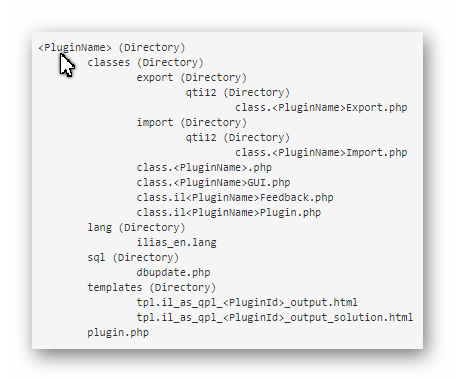
\includegraphics[page=1, width=0.3\paperwidth, trim=4 4 4 4, clip]{fig/ILIAS-Dateistruktur.png} 
            \caption{Dateistruktur eines ILIAS Frageplugins (aus \cite{IliasDevelopmentGuide}, Kapitel 26)}
            \label{fig:ilias-dateistruktur}
        \end{center}
    \end{figure}
    
    Da der Development-Guide keine Methoden und Klassen der Schnittstelle beschreibt, ist es sehr hilfreich, dass mit der \eigenname{assExampleQuestion} eine beispielhafte Implementierung eines Plugins verlinkt ist (s. \cite{AssExampleQuestion}), die die Basis-Methoden eines auf der \eigenname{ILIAS} Plugin-API aufsetzenden Fragenplugins zeigt. Noch mehr Methoden samt ihrer Verwendung werden in weiteren veröffentlichten Plugins, wie der \eigenname{assCodeQuestion} gezeigt (s. \cite{AssCodeQuestion}).

\subsection{SQL.js}
\label{subsec:sql-js}

    \eigenname{SQL.js} ist - wie bereits oben erläutert - eine als Javascript kompilierte Version des Datenbanksystems \eigenname{SQLite}. Die Kompilierung von \eigenname{SQL.js} ist durch \eigenname{Emscripten} (s. \cite{Emscripten}) erfolgt und bietet somit die in \eigenname{SQLite} verfügbare \eigenname{SQL} Logik. Ein großer Unterschied zu \eigenname{SQLite} ist es jedoch, dass Daten in \eigenname{SQL.js} nicht persistent gespeichert werden. Das erneute Laden einer Seite führt zu einer frischen Instanz von \eigenname{SQL.js}.
    
    Weitere Informationen zu \eigenname{SQL.js} finden sich unter \cite{SQLjs}. Dabei wird auch auf eine kurze, aber hilfreiche Dokumentation aller Funktionen von \eigenname{SQL.js} hingewiesen (s. \cite{SQLjsDocu}), sowie eine Reihe an Beispiel Implementierungen verlinkt (s. \cite{SQLjsExa}). Unter anderem ist eines der dort aufgeführten Beispiele ein \eigenname{Online SQL Interpreter}, dessen Ideen zu Parallelisierung die Basis für die Implementierung von \eigenname{SQL.js} im \eigenname{QPI-SQL} Projekt gegeben haben.